\subsubsection{Survey Results}

Near the end of the first trial, the LinkR users were invited to
answer a survey regarding their experiences with the recommendations
they were getting. They were asked a number of questions, with the
following pertaining to the quality of the recommendations:

\begin{itemize}
\item{Do you find that ANU LinkR recommends interesting links that you may not have otherwise seen?}
\item{Do you feel that ANU LinkR has adapted to your preferences since you first started using it?}
\item{How relevant are the daily recommended links?}
\item{Overall, how satisfied are you with LinkR?}
\end{itemize}

They gave their answers to each question as an integer rating with
range $[1-5]$, with a higher value being better. Results are shown in
Figure~\ref{fig:survey1}. Their answers were grouped together
according to the recommendation algorithm that was assigned to them,
and the averages per algorithm are below.

As shown in Figure~\ref{fig:survey1}, Social Matchbox achieved higher
survey scores than the other recommendation algorithms, in all four
questions. The results of the survey reflected the results in the
online live trial and confirms that Social Matchbox was the best
recommendation algorithm in the first trial.
 
\begin{figure*}[t!]
\centering
\subfigure{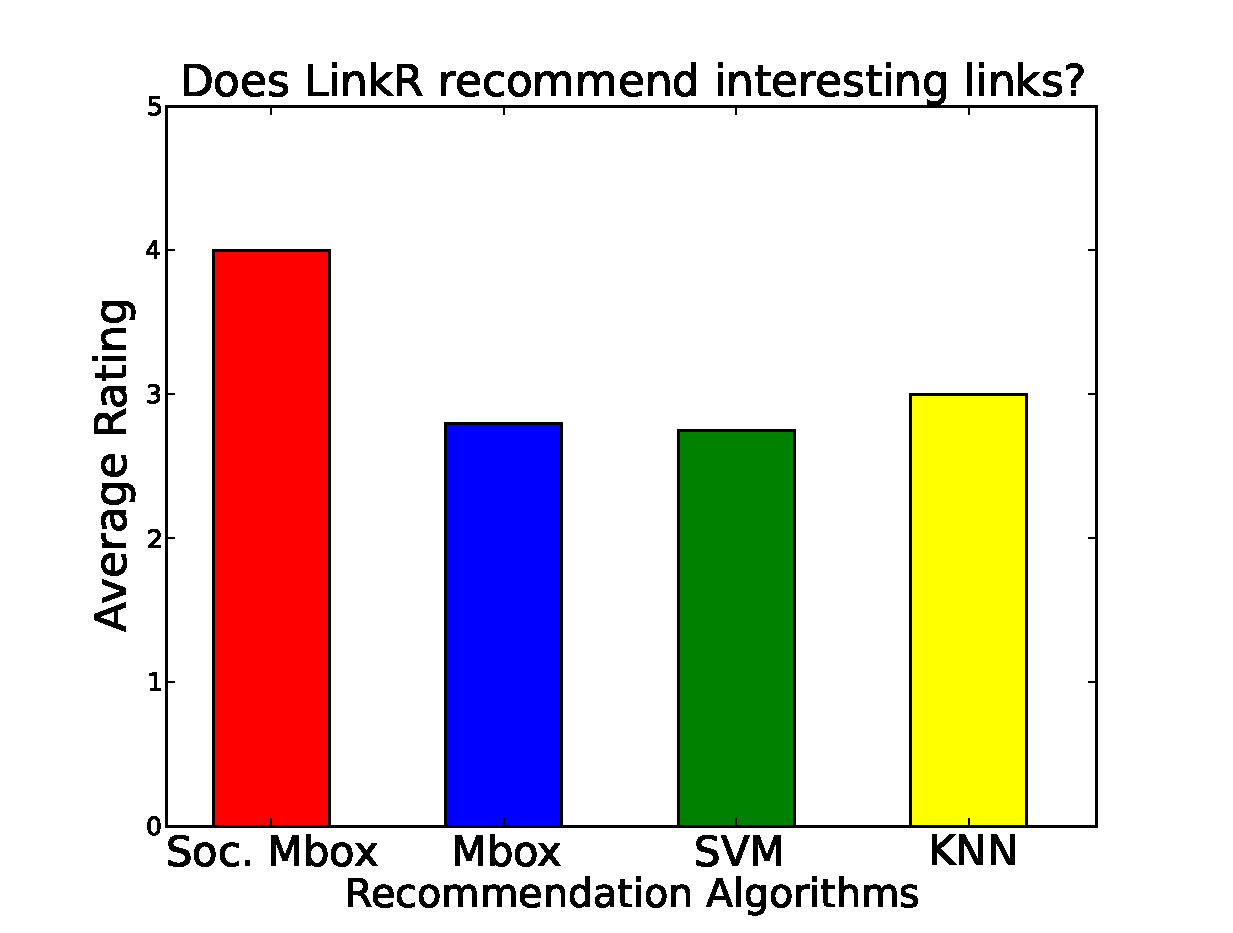
\includegraphics[scale=0.23]{img/not-seen.eps}}
\hspace{-6mm} \subfigure{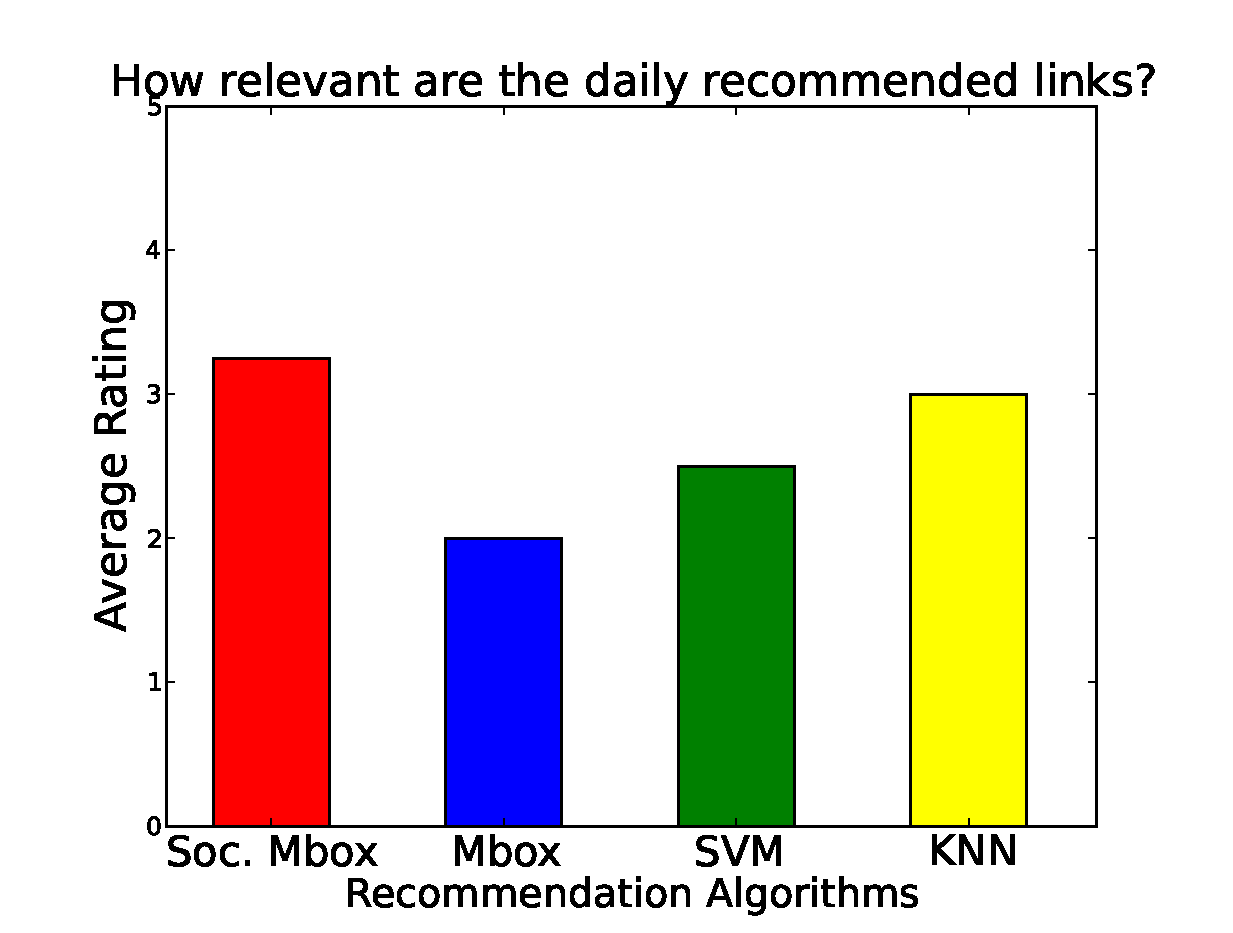
\includegraphics[scale=0.23]{img/relevant.eps}}
\hspace{-6mm} \subfigure{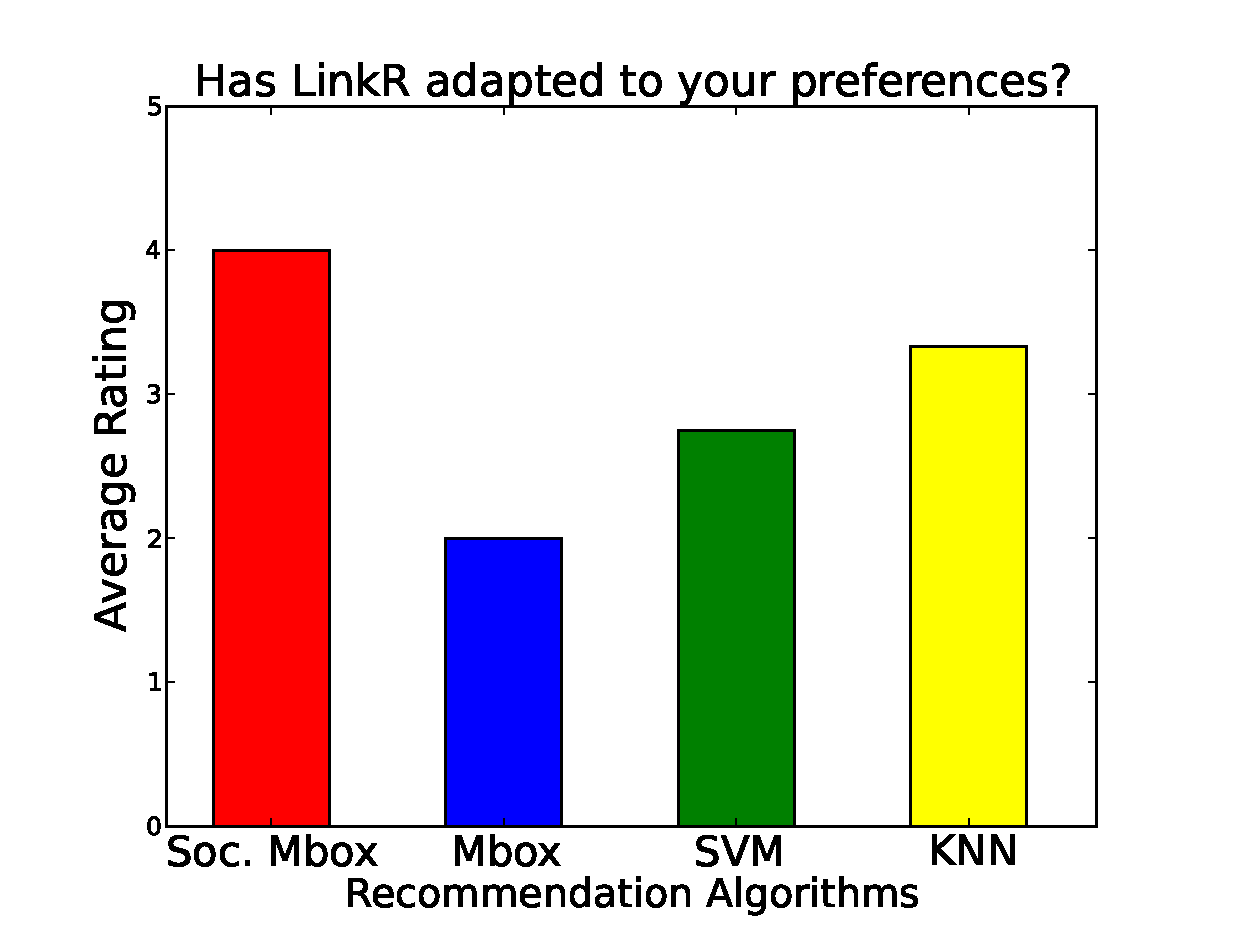
\includegraphics[scale=0.23]{img/adapted.eps}}
\hspace{-6mm} \subfigure{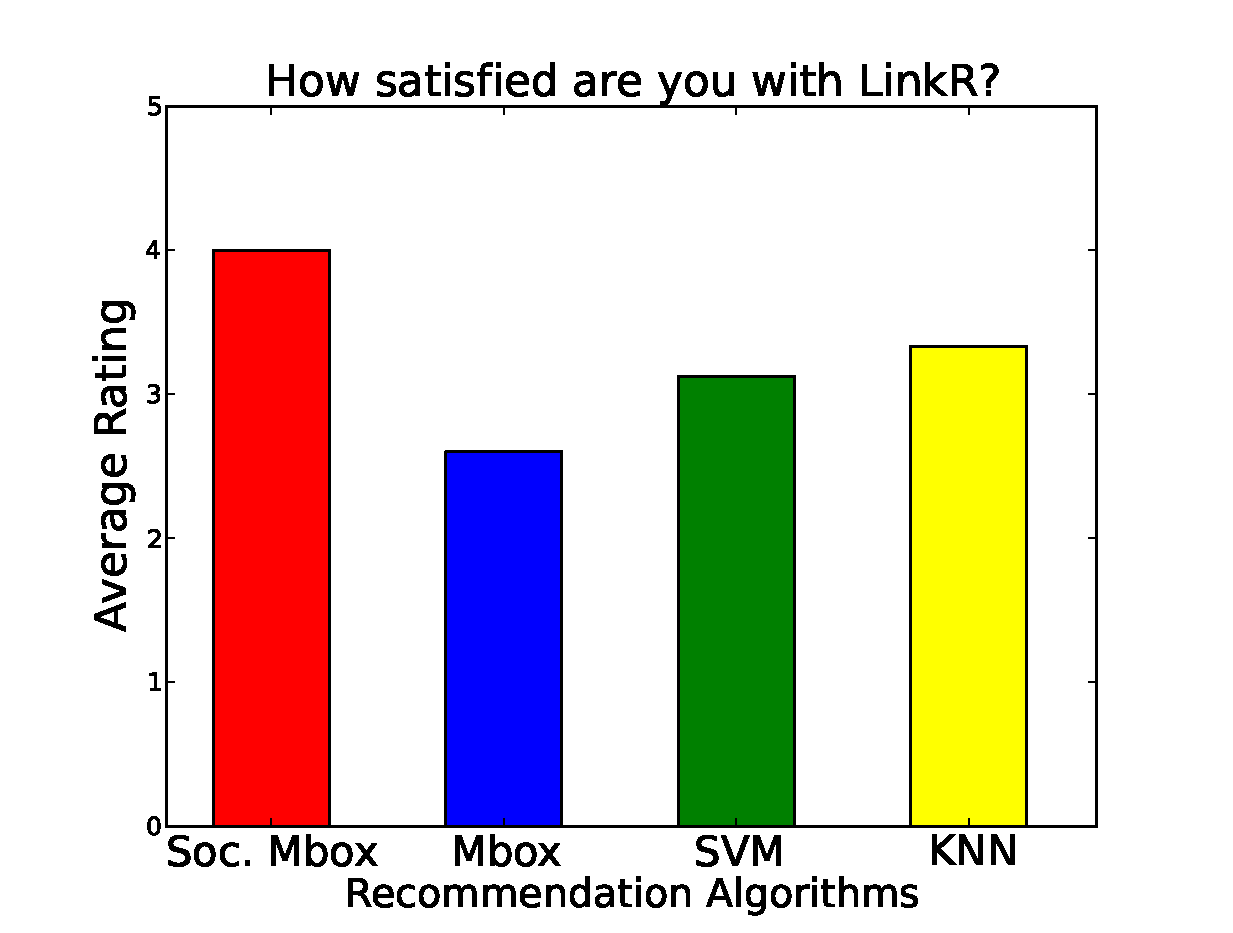
\includegraphics[scale=0.23]{img/satisfied.eps}}
\caption{Results of the user survey after the first trial. The survey answers from the users reflect the online results that Social Matchbox was the best recommendation algorithm in this trial.}
\label{fig:survey1}
\end{figure*}
